\newpage\null\thispagestyle{empty}\newpage
\clearpage{\thispagestyle{empty}\cleardoublepage}
\part{Software}
% \acbarrier
\parttoc
% 
% 
% 
\setcounter{chapter}{3}
\chapter{Nerve fiber modelling}
\label{chap:sof:modelling}
% 
In \cref{chap:neuro} both the structure of nerve fibers and the macroscopic structure of \ac{WM} were described.
The question is how to represent such a structure in a computer algorithm?
For simple fiber configurations, \eg{} parallel, linear nerve fibers, this is quite straightforward.
However, it has been shown that irregular, non-symmetric nerve fiber configurations are necessary to obtain a realistic result for microscopy simulations based on the wave nature of the light \cite{MenzelDissertation}.
Therefore one needs ideally a representation, which allows to build any kind of pattern.
\par
%
Many solutions are already available.
A common one is used in graphical visualizations.
A rope or fiber, \ie{} a raw object, is defined by a trajectory with a radius.
From this, a surrounding mesh is generated.
In visualization, the mesh is used to apply textures to represent a surface.
Such meshes are \eg{} used in Monte Carlo simulations of \ac{dMRI} \cite{Ginsburger2019,ginsburgerDis2019}.
In this type of simulation, the meshes help calculate whether a water molecule travels through the surface of a nerve fiber, i.e., the surface of the mesh.
However, this representation is very computationally intensive because the number of triangles that must be present in the mesh is quite high.
\par
%
When creating complex nerve fiber structures, it is important that the nerve fibers do not overlap.
In simulations in which the wave nature of light is modeled, this otherwise leads to significantly altered results.
To achieve non overlapping fibers, either the user must define such a structure in advance, or a computer algorithm must build such structures automatically.
Considering the immense number of configuration possibilities that nerve fibers can have even in a small volume, the task is almost impossible for a user to solve except for trivial configurations.
The same is true for a computer algorithm.
One could write an algorithm that defines a single fiber in a volume and then places the next one, making sure that none overlaps and so on.
This works well up to a point.
Even if an algorithm always finds a solution to find a path through an partially filled volume, at some point the volume will appear to be full, but still have plenty of free space between fibers.
Of course, one can minimize this behavior by trying to place nearly parallel fibers, but again, looking at real tissue data, \eg{} \cref{fig:brainTPFM,fig:elecMic}, this does not reflect reality.
Even in a fiber bundle, the fibers are so densely packed that you can't just add another fiber in a way that wastes volume over time (\ie{} add more fibers).
\par
%
The solution found in this work is to allow the placement of nerve fibers in any way and without any restriction.
The overlap will be removed in the folliwing step.
Check all fibers for collisions with each other.
If a collision occurs, try to remove it by moving the colliding parts slightly away from each other.
Repeat this step until all collisions are removed.
\par
%
This idea with all its necessary prerequisites is described in detail in the following chapter.
First, the representation of a nerve fiber is defined in a way that it already takes into account to be as performant as possible for the collision process.
Then, additional \textit{building} functions are designed to help the user quickly define a volume with nerve fibers.
Finally, the algorithm for resolving the collisions with the parallelization components is explained in detail.
In addition, another approach based on this idea and developed in this work with colleagues from \ac{dMRI} is explained in detail.
This one focuses on the placement of neurons such as astrocytes or olegodendrocytes in a volume with fibers.
The collaboration is possible since both simulation techniques study the same type of tissue models.
Since these models focus on non-overlapping tubular structures, they can also be applied to other fibrous structures such as skeletal muscle fiber \cite{Ji2021}.
\par
%
All described algorithms here are part of the toolbox \ac{fastPLI} \cite{Matuschke2019, Matuschke2021}, which is described in detail in \cref{chap:Software}.
The original idea of a collison free algorithm is published in \cite{Matuschke2019}.
%
%
%
\section{Nerve fiber representation}
\label{sec:nerve_fiber_representation}
%
Nerve fibers themselves are tube-like structures surrounded by an electrically insulating lipid layer of myelin (see \cref{sec:fiberArchitecture}).
Both the diameter of the axon and the thickness of the myelin can vary greatly from fiber to fiber (see \cref{sec:axonMicroscopy}).
This means that the representation of nerve fiber models should be able to represent such variations as well.
\par
%
As described in \cref{sec:fiberArchitecture} \ac{WM} consist of nerve fibers packed tightly together in nerve fiber bundles.
These bundles can join with other bundles and traverse the brain to connect one region to another.
The bundles are able to cross each other, either by crossing the individual nerve fibers or bypassing the fiber bundles.
This can \eg{} generate interwoven structures.
Such structures are a key element in the study of \ac{3D-PLI}.
Therefore, it is particularly important that the models are able to form such structures without overlapping individual fibers.
\par
%
One way of representing individual nerve fibers is a parametric function describing a path in 3d space, \ie{} a trajectory.
In addition, a fourth element describes the radius of the fiber at the same point:
% 
\begin{align}
f(t) \rightarrow (x(t),y(t), z(t), r(t))
\end{align}
% 
However, this representation does not allow simple subsequent changes, such as resolving collisions.
For this purpose, individual elements are more manageable, allowing movement or deformation.
Therefore, the function or fiber is divided into smaller discrete segments.
%
\begin{figure}[!t]
    \setlength{\tikzwidth}{0.85\textwidth}
    \centering
    % \tikzset{external/export next=false}
    \inputtikz{gfx/model/fiber_model}
	\caption[]{Representation of a nerve fiber from a list of spheres.}
	\label{fig:fiberReb}
\end{figure}
%
Therefore, the fiber can be described by a list of 4d points $(x,y,z,r)$, which can be interpreted as a chain of cylindrical fiber segments (see \cref{fig:fiberReb}):
\begin{align}
\begin{gathered}
\mathit{fiber} = \left\{ \vec{p}_i=(x_i,y_i,z_i), r_i \mid x,y,z \in \mathbb{R}, \, r \in \mathbb{R^+}, \, i \in \{0,1,...,N_{\mathit{points}}-1\}\right\} \\
\mathit{fiber\_segment}_i = (\vec{p}_i, \vec{p}_{i+1}, r_i, r_{i+1}), \, i \in \{0,1,...,N_{\mathit{points}}-2\}
\end{gathered}
\end{align}
%
\begin{figure}[!t]
    \centering
    \setlength{\tikzwidth}{0.5\textwidth}
    \inputtikz{gfx/model/capsule}
	\caption{Schematic of a fiber segment represented by a  \acreset{CC} \ac{CC}}
	\label{fig:conical}
\end{figure}
%
Since the fiber radius can change from one point to an adjacent point, the segment can be conical.
Therefore, the fiber segments describe a \ac{CC} (see \cref{fig:conical}).
\par
%
This representation has the advantage over a mesh representation of a surface that much less data is needed for the representation.
This will increase the computational speed, which will be crucial for a collision solving algorithm.
%
% 
% 
\section{Sandbox}\label{sec:sandbox}
%
In computer game terminology, a \textit{sandbox mode} is a game mode that allows the player to build and design anything at no cost.
Analogous to this feature is the \pymodule{fastpli.model.sandbox}, which allows the user to easily and quickly design standard geometric configurations of nerve fibers and bundles.
Since nerve fibers are usually arranged in bundles, the design methods focus on generating nerve fiber bundles from a 2d pattern (seed points) and a nerve fiber bundle trajectory.
\par
%
This module is divided into two successive submodules.
The first module handles the seeding process, while the second part builds up a nerve fiber bundle or volume filled with individual fibers from seed points.
%
\subsection{Seeding fiber bundles}\label{sec:seeds}
%
\begin{figure}[!t]
    \def\tikzheight{0.25\textwidth}
    \centering
    \subcaptionbox{\label{fig:triGrid}equilateral triangle grid}[.32\textwidth]{
    \inputtikz{gfx/model/triangular_grid}}
    \hfill
    \subcaptionbox{\label{fig:rndGrid}random grid}[.32\textwidth]{
    \inputtikz{gfx/model/rnd_circle_points}}
    \hfill
    \subcaptionbox{\label{fig:crossBundle}populated fiber bundles}[.32\textwidth]{
    \inputtikz{gfx/model/crossing_bundle}}
	\caption{Populating fiber bundles with 2d seed points.}
% 	\label{fig:}
\end{figure}
%
Seed points are stored as a list of 2d points:
\begin{align}
\mathit{seeds} = \left\{ \vec{p}_i=(x_i,y_i) \mid x,y \in \mathbb{R} , \, i \in \{0,1,...,N_{\mathit{seed\_points}}-1\}\right\}
\end{align}
%
To form particularly dense fiber bundles, a method for generating an equilateral triangular grid is implemented (see \ref{fig:triGrid}).
Mathematically, this yields the most densely packed pattern for a 2d circle with equal radius packed area.
However, this very regular symmetric grid can lead to unrealistic results (\eg{} diffraction pattern in light wave simulation \cite{MenzelDissertation}).
It should therefore only be used as an initial configuration.
Since the initial configurations are often unknown, it is probably best to choose a random distribution (see \cref{fig:rndGrid}).
For a circular boundary, this is done with:
% 
\begin{equation}
\begin{split}
\varphi &= \mathrm{uniform}(0,2 \pi) \\
r &= R \sqrt{\mathrm{uniform}(0,1)}
\end{split}
\quad\Rightarrow\quad
\begin{split}
x = r \cos(\varphi)\\
y = r \sin(\varphi)
\end{split}
\end{equation}
%
%
%
\subsection{Populating fiber bundles}\label{sec:fillBundle}
%
\begin{figure}[!t]
    \centering
    \setlength{\tikzwidth}{0.75\textwidth}
    \inputtikz{gfx/model/min_torsion}
	\caption{Left: Plane of seed points. Right: Plane are rotated and placed along the path. At the end, the plane has the same normal vector as the starting plane, but due to the principle of minimum rotation, the plane is rotated along the normal vector.}
	\label{fig:torsion}
\end{figure}
%
To populate a fiber bundle, the plane containing the seed points is placed at each fiber bundle point $\vec{fb}_i$ along the trajectory.
Essentially, for each resulting $\mathit{fiber}_j$, this means:
% 
\begin{align}
    \mathit{fiber}_j = \left\{ \mat{R} \cdot (x_j, y_j, 0) + \vec{fb}_i \, | \, i \in \{0,1,...,N_{\mathit{seed\_points}}-1\}\right\}
\end{align}
% 
However, the question is which rotation matrix $\mat{R}$ has to be applied.
Since a trajectory is only a 2d object, \ie{} a line, no unique normal vector can be defined in space.
In mathematics, the torsion of a curve can be defined with a principal normal vector and a binormal vector.
However, this has the problem that a line such as a helical function has a torsion, \ie{} the line rotates along its path.
This would mean that the individual fibers would rotate around the path of the fiber bundle if the seed point plane were placed according to the principal and binormal vectors.
This is possible in principle, but practically non-existent in real tissue.
\par
% 
A more reasonable solution is to perform a rotation such that the rotation along the fiber bundle trajectory is minimal.
This can be achieved by computing the rotation matrix that would rotate the current tangent vector $\vec{t}(i)$ to that of the nearest point $\vec{t}(i+1)$.
The rotation matrix $\mat{R}(\vec{a}, \vec{b})$ can be calculated, except for $\vec{a} || \vec{b}$ via
\begin{align}
\begin{split}
    \vec{a} =& \; \vec{a} / |\vec{a}|\\
    \vec{b} =& \; \vec{b} / |\vec{b}|\\
    \vec{v} =& \; \vec{a} \times \vec{b}\\
    c =& \; \vec{a} \cdot \vec{b}
\end{split}
\quad
\begin{split}
    \mat{U} =& \begin{pmatrix} 0 & \vec{v}_z & -\vec{v}_y\\ -\vec{v}_z & 0 & \vec{v}_x\\ \vec{v}_y & -\vec{v}_x & 0\end{pmatrix}\\
    \mat{R} =& \; \mathbb{1} + \mat{U} + (\mat{U} \cdot \mat{U}) \cdot (1 - c) / |\vec{v}|^2
\end{split}
\end{align}
% 
In the case of $\vec{a} || \vec{b}$ no roation is necesarry.
\par
% 
This tool enables the following procedure:
First, place the seed point plane at the first fiber bundle point $\vec{fb}_0$ and rotate it by $\mat{R}(\hat{\vec{e}}_z, \vec{t}_0)$.
Then, for each step, the plane is rotated at its original origin according to $\mat{R}(\vec{t}_i, \vec{t}_{i+1})$ and placed on $\vec{fb}_{i+1}$.
To smooth the transition, the tangential vector at step $i$ is calculated as follows.
\begin{align}
    \vec{t} = \frac{1}{2} \frac{\vec{fb}_{i-1} + \vec{fb}_{i+1}}{|\vec{fb}_{i-1} + \vec{fb}_{i+1}|}
\end{align}
%
Finally, all points belonging to a fiber can be stored in a fiber bundle object as $(n \times 4)$-array.
% An example is shown in \cref{fig:bendingFiberBundle}.
%
%
%
\subsection{Cube models} \label{sec:cubeModelBuilding}
%
\begin{figure}[!t]
    \centering
    \setlength{\tikzwidth}{0.5\textwidth}
    \inputtikz{gfx/model/cube_build}
	\caption{Populating a cuboid with straight fibers initialized by seed points along the direction $\vec{v}$.}
    \label{fig:cubeBuild}%
\end{figure}
%
As will be shown later, the \ac{3D-PLI} simulation wil calculate a image based on a cubical volume.
Therefore, a method exists to fill such a volume with a fiber population of orientation $\vec{v}$ (see \cref{fig:cubeBuild}).
The individual fibers are initialized as usual with a seed point plane.
This plane is virtually placed in front of the cubic volume end behind it in the direction of the orientation, so that the origins of the seed point planes coincide with the origin of the cube.
Then the seed points are virtually connected.
When a line meets the volume, the entry and exit points are calculated and stored as fibers of the fiber bundle.
%
%
%
\subsection{Cylindric models}
%
\begin{figure}[!t]
    \centering
    \setlength{\tikzwidth}{0.31\textwidth}
    \subcaptionbox{\label{fig:cylCircular}%
        Circular population.
    }[.33\textwidth-1ex]{
    \inputtikz{gfx/model/cylinder_circular}}\hfill
    %
    \subcaptionbox{\label{fig:cylRadial}%
        Radial population.
    }[.33\textwidth-1ex]{
    \inputtikz{gfx/model/cylinder_radial}}\hfill
    %
    \subcaptionbox{\label{fig:cylParallel}%
        Parallel population.
    }[.33\textwidth-1ex]{
    \inputtikz{gfx/model/cylinder_parallel}}
	\caption{Populating of cylindrical objects. The green area shows the area corresponding to the seed points in the xy-plane. The coordinate system indicates the coordinate origin coresponding to the seed points origin.}
\end{figure}
%
The last method allows to populate a cylindrical volume with fibers.
Since a cylinder has three symmetries, a radial, an angular and the length, those three methods have been implemented to provide a way to populate the volume.
\par
%
First, the coordinate system must be defined.
The cylinder with outer radius $r_{\mathit{out}}$ and inner radius $r_{\mathit{in}}$ is aligned along the z-axis with height $h$ and starts at $(0,0,0)$.
In addition, the cylinder can be cut radially at a directional angle $\alpha$ to $\beta$ to fill only a portion of it.
The angles corresponds to the cylindrical coordinate system of the resulting model.
\par
%
The following applies to all methods used: If the seed point plane leaves the cross-section plane to be filled, the seed points lying outside are ignored.
%
\paragraph{a) circular}
Mimics a radial path of the cylinder (see \cref{fig:cylCircular}).
The seed points are placed along the surface of the cross section of the first $\alpha$ direction angle.
The origin of the seed point plane is placed on the origin of the cylinder.
From there, the fiber is circular to the second $\beta$ direction angle.
The step size of the circular path can be costamized.
%
\paragraph{b) radial}
The fibers are placed from the inner wall to the outer wall of the cylinder.
The seed point plane is therefore placed at the inner wall with the origin at the bottom corner of the first angle $\alpha$ (see \cref{fig:cylRadial}).
The fibers are then generated radially until they meet the outer wall of the cylinder.
Thus, the density of the fibers decreases along their path.
%
\paragraph{c) parallel}
The fibers are aligned along the cylinder (see \cref{fig:cylParallel}).
Here, the seed points are in the lower plane, with both coordinate origins in the same point (see \cref{fig:cylParallel}). The orientation of the plane is aligned with the x-axis at $\SI{0}{\degree}$
%
%
%
\section{Solving fiber collisions}
\label{sec:Solver}
%
The focus of the following algorithm is to allow the user to define any fiber path.
This allows a wide range of freedom in the initialization process.
Of course, since the fibers are 3d volume objects,  there will probably overlaps with other fibers.
The aim of the following algorithm is to find and solve such collisions by moving the affected fiber segment in such a way that a collision-free volume is created by minimal displacement.
This allows the user to specify complex interwoven structures such as nerve fiber crossings in a fairly straightforward manner.
Additionally the algorithm allows the user to specify boundary conditions like the mean fiber segment length or minimal bending radius.
\par
% 
An important feature is the visualization of the solution process.
This allows the user to see what is happening and intervene as early as possible if necessary.
This is very important because the solution process can take a lot of time, depending on the volume and the number of objects.
%
%
% 
\subsection{Solver main}
%
\begin{lstfloat}[!tb]
\lstset{style=python}
\begin{lstlisting}[]
def step():
    # Reset Parameter
    SetSpeed(objects, 0)
   
    # Building Octree
    octree = Octree(objects)
   
    # Collision Detection
    for leaf in octree:
        colliding_objs = CheckLeaf(leaf.fiber_list)
        colliding_list.insert(colliding_objs)

    # Seperation Process
    MoveObject(colliding_list)

    # Shape Control
    SegmentLength(colliding_list, target_length)
    BendingRadius(colliding_list, target_curvature)

    return colliding_list.is_empty()
\end{lstlisting}
\caption{Main structure in a single step of the collision checking and shape controlling algorithm.}
\label{alg:pseudocode_solver}
\end{lstfloat}
%
Apart from the initialization of the parameters, the main function of the solver algorithm is a computational \code{step} of the solution procedure.
The algorithm is with reason not a loop by itself.
This allows the user to interact with the data or parameters at each step, if necessary.
This \code{step} function (see \cref{alg:pseudocode_solver}) can be divided into the following sequential parts:
Ordering the objects in a octree, checking each branch of the octree for colliding objects, separating the colliding objects, and checking the shape of the fibers.
The return value of the function is a boolean if no colliding objects were found.
A stand-alone algorithm is published in \cite{Matuschke2019}.
At this point it is integrated into the \ac{fastPLI} package under \pymodule{fastpli.model.solver.Solver}.
%
%
%
\subsection{Collision Detection}
\label{sec:collisionDetection}
%
\begin{figure}[!t]
    \centering
    \setlength{\tikzwidth}{0.75\textwidth}
    \inputtikz{gfx/model/conical_capsule_bb}
    \tikzset{external/export=false}
	\caption[]{Fiber segment representations with the \acp{AABB}: \raisebox{.25em}{\tikz \draw[black](0,0)--(0.275,0);} \ac{CC}, \raisebox{.25em}{\tikz \draw[blue, dash pattern=on 2.5pt off 2.5pt](0,0)--(0.275,0);} capsule, \raisebox{.25em}{\tikz \draw[red, dash pattern={on 2.5pt off 0.9pt on 0.42pt off 0.9pt}](0,0)--(0.275,0);} bounding box.}
	\label{fig:conical_capsule}
\end{figure}
% 
As described in \cref{sec:nerve_fiber_representation}, nerve fibers are represented as a chain of spheres, with two adjacent spheres combined into a fiber segment that forms a \ac{CC} (see \cref{fig:conical_capsule}).
To simplify the calculation, only the \acp{AABB} is initially checked for collision.
%
\begin{lstfloat}[!tb]
\lstset{style=python}
\begin{lstlisting}[]
def aabb_collide(aabb_0, aabb_1):
  for i in dim(aabb):
      if aabb_0[i].min > aabb_1[i].max:
         return false
      if aabb_0[i].max < aabb_1[i].min:
         return false
  return true
\end{lstlisting}
\caption{Calculation if a collission between \acp{AABB} exists.}
\label{alg:collisionAABB}
\end{lstfloat}
%
This check is quite simple and involves only a few steps (see \cref{alg:collisionAABB}).
If a collision occurs between the two \acp{AABB}, the next more precise collision check is performed.
However, this is a non-trivial task and very computationally intensive.
Therefore, it was decided to change the object representation for the collision detection part from a \ac{CC} to a capsule (see \cref{fig:conical_capsule}).
This means that the radii of the \ac{CC} for both spheres grow to the maximum of the two spheres $r_{\mathit{capsule}} = \mathrm{max}(r_0, r_1)$.
This has the obvious disadvantage that space is lost. However, for small changes in radii, this is a great advantage in terms of computational cost.
\par
% 
\begin{lstfloat}[!t]
\resizebox{\textwidth}{!}{
% \begin{sideways}
\begin{tabular}{|cc|cc|}
\hline
\hspace{1em} &
\begin{minipage}{0.4625\textwidth}
\lstinputlisting[style=python,basicstyle=\scriptsize\ttfamily,firstline=1,lastline=32]{code/collision_detection.py}
\end{minipage} & \hspace{1em} &
\begin{minipage}{0.4625\textwidth}
\lstinputlisting[style=python,basicstyle=\scriptsize\ttfamily,firstline=33,lastline=64,firstnumber=35]{code/collision_detection.py}
\end{minipage} \\
\hline
\end{tabular}
% \end{sideways}
}
\caption{Collision detection between two capsule objects. A collision occurs if the distance is less than $\mathit{cone_a.r}+\mathit{cone_b.r} > d$.}
\label{alg:pseudocodeCollisionDetection}
\end{lstfloat}
% 
The algorithm for detecting collisions between two capsules is described in \cref{alg:pseudocodeCollisionDetection}.\footnote{\href{https://www.john.geek.nz/2009/03/code-shortest-distance-between-any-two-line-segments/}{https://www.john.geek.nz/2009/03/code-shortest-distance-between-any-two-line-segments/}}
%
\begin{figure}[!t]
    \centering
    \def\tikzheight{0.5\textwidth}
    \inputtikz{gfx/model/shortest_dist}
	\caption{Shortest distance between two capsule objects. The line must be either perpendicular to the line segments or at least in one of the points of each object.}
	\label{fig:shortDist}
\end{figure}
%
It works on the principle that it calculates the shortest distance between two line segments.
Three cases can occur.
First, the shortest distance is a line perpendicular to the two line segments (see \cref{fig:shortDist}).
Second, only one line segment is perpendicular to the shortest distance line.
The other has an anchor point either at the beginning or at the end of the second line segment.
Third, the shortest distance is a connection between one of the points of the line segments.
For cones, a collision occurs when the distance is less than the sum of the two radii.
\par
% 
It can be assumed that the calculation of the collision check will be the most complex function at this point.
Therefore, the next step is to reduce the amount of computation as much as possible.
An initial naive collision check would compare each object to all other objects.
The next object must then be checked against $n-1$ and so on.
This leads to a computational cost of $\mathcal{O}(n^{2})$, which is not acceptable for large n.
Therefore, another strategy must be chosen to reduce the number of computations.
%
% 
% 
\subsection{Octree}\label{sec:octree}
%
\begin{figure}[!t]
    \centering
    \subcaptionbox{\label{fig:octreeCube}Exemplary octree subdivision of a cube.}[.3\textwidth]{
    \def\tikzheight{0.6\textwidth}
    \inputtikz{gfx/model/oct_tree}}
    \hfill
    \subcaptionbox{\label{fig:collision2D}Exemplary collision in 2d. The \textcolor{RED}{boxes} corresponds to the \acp{AABB} }[.65\textwidth]{
    \def\tikzheight{0.6\textwidth}
    \inputtikz{gfx/model/collision_tree}}
	\caption{Exemplary tree subdivision.}
	\label{fig:octree}
\end{figure}
%
A \name{tree} is a data structure consisting of a collection of \name{nodes} that are connected to each other.
A \name{node} is connected to a single parent \name{node}, and to multiple \name{children} via \name{branches}.
The first parent node is called \name{root}.
The final \name{nodes} at the end of a \name{branch} are called \name{leafs}, which contain the data.
Traversing a uniformly distributed \name{tree} has the advantage that the cost of traversal is $\mathcal{O}(\log(n))$.
\par
%
An \name{octree} is a special kind of \name{tree} where each node contains eight children.
This allows a cubic volume to be divided into eight subvolumes, which in this case are of equal size.
An example is shown in \cref{fig:octreeCube}.
This means that the length of the volumes shrinks exponentially with $(1/2)^\mathit{level}$.
An \name{octree} can be implemented in several ways.
Here, a recursion function was chosen (see \cref{alg:pseudocode_octree}), which is a function which that calls itself.
%
\begin{lstfloat}[!tb]
\lstset{style=python}
\begin{lstlisting}[]
def octree(volume, objects):
    if num(objects) > threshold:
        sub_volumes, sub_objects = split(volume, objects)
        leafs = [octree(v,o) for v,o in zip(sub_volumes, sub_objets)]
    else:
        leafs = [objects]
    return leafs
\end{lstlisting}
\caption{Generation of an octree.}
\label{alg:pseudocode_octree}
\end{lstfloat}
%
The idea of tree generation is the following:
At the beginning, all objects must be sorted into the eight \name{leafs} of the current node (if the number of objects is not too small).
This means that for each object it must be checked whether there is a collision with one or more of the eight \name{leafs}, \ie{} the cubic subvolumes.
However, since this already implies a high checking effort, the checking function should be as fast as possible.
For this purpose, analogous to the object collision check (see \cref{fig:collision2D}), only the \ac{AABB} of the object is checked for collision with the leaf volume, which is also a \ac{AABB}.
This means that there may be cases where an object is placed in a subvolume to which it does not belong.
However, in this case, the increasing speed of the checking process is an advantage.
Once all objects are sorted into their respective subvolumes, recursion can begin.
Since a branch can be considered a node, the same algorithm can be executed until a desired boundary or property is reached, \ie{} recursive execution.
This means that the current (sub-)volume is split into eight subvolumes again, if necessary, and the objects of the current (sub-)volume are sorted into the new subvolumes.
The recursion also means that the next function call must contain a list of the current objects.
This means that the objects must either be copied, which is time consuming, or referenced by \eg{} and index, which is aso time consuming because the data is accessed randomly in memory.
The first option was chosen because it proved to be the fastest in a speed test during implementation.
The next question is what is the desired goal to end the branching process and mark the node as a leaf and therefore the collision checking algorithm can be applied between all objects in each leaf.
\par
%
The goal is to reduce the computation time.
Unfortunately, with a structure like an octree, there is no straightforward way to give a definitive answer.
It depends on the scope and the contained objects themselves.
For example, if all the objects overlapped, all the objects would be sorted into all the leaves and thus eight times as much would be tested.
This is of course an extreme case, but depending on the user's input, can occure.
The user should therefore separate the fibers as much and as sensibly as possible during initialization.
The usual approach is to impose the following two constraints:
%
\paragraph{Maximum number of levels}
In the case of nerve fibers, it can be assumed that the size of the objects is approximately in the same order of magnitude.
This means that the largest object in a volume can be used as the lower bound for the smallest volume in the octree.
In the case of object sizes that differ in higher orders of magnitude, this will consequently increase the computational cost to the point where each object must be retested with each object.\footnote{There are other, more suitable algorithms for this case. However, since this case is not expected, they are not implemented}.
%
\paragraph{Minimal number of objects}
Once a \name{leaf} could be created, all objects contained in it must be checked for collisions.
As mentioned above, this is a task of $O(n^2)$.
However, there is also an upper bound of a number of objects for which it is faster to calculate whether they collide than to further partition the volume.
This number must be checked at runtime, since it depends on many factors.
In the development phase of this algorithm, a value of $\approx \SI{20}{}$ for the involved computer architectures could be determined.
\par
%
At this point the collision checking algorithm is performent on each leaft (see \cref{sec:collisionDetection}) and all colliding objects are be identified.
The next step is to change their positions so that their collision is reduced or completely separated.
%
\subsection{Separation Phase}
% 
To resolve a collision between two \ac{CC} objects, each point $\vec{p}_i$ and $\vec{p}_{i+1}$ of the two objects is moved.
To effective move the objects aport with a small effort, the fiber objets are translated and rotated away from the other coliding object.
The translation is parallel to the shortest distance vector of the collision.
For the rotation the direction of motion is weighted by the distance of each point from the intersection with the smallest distance line (see \cref{fig:shortDist,alg:push_apart}).
% 
\begin{lstfloat}[!h]
\lstinputlisting[style=python]{code/push_apart.py}
\caption{Velocity calculation of coliding objects.}
\label{alg:push_apart}
\end{lstfloat}
% 
% \begin{align}
% v_i = \dummy{}
% \end{align}
\par
%
The velocity is stored in an array for each fiber corresponding to the fibers points.
All velocities for a single point will be summed up.

\par
% 
A special case is the movement of the first and last point of a fiber.
These may only move perpendicular to the first/last segment line.
This prevents the fibers from growing to infinity.
% 
% 
%
\section{Shape control}\label{chap5:ShapeControl}
% 
The movement of single points can lead to a distorted fiber model, \eg{} two points move very far apart.
Therefore, boundary conditions are specified.
It was decided to use the following two properties, the mean segment length and the minimum bending radius, as parameters for the shape control.
Each parameter can be set to $\SI{0}{}$ to disable the boundary condition.
%
% 
% 
\subsection{Mean segment length}
%
\begin{figure}[!t]
    \centering
    \setlength{\tikzwidth}{0.75\textwidth}
    % disable tikz externalize for overlayed circle lines
    % \def\forcetikzscale{true}
    % \tikzset{external/export=false}
    \inputtikz{gfx/model/model_length}
	\caption{Different fiber segment lengths as factor of the mean fiber radius $\fiberRadiusMean$.}
	\label{fig:modelLength}
\end{figure}
%
\begin{figure}[!t]
    \centering
    % \tikzset{external/force remake}
    \tikzset{external/export=false}
    \def\forcetikzscale{true}
    \setlength{\tabcolsep}{0pt}
    \setlength{\tikzwidth}{.45\textwidth}
    \begin{tabular}{C{.5\textwidth}C{.5\textwidth}}
    \inputtikz{gfx/model/model_merge} &
    \inputtikz{gfx/model/model_split} \\
    \subcaptiontab{0.475\textwidth}{merge} &
    \subcaptiontab{0.475\textwidth}{split}
    \end{tabular}
	\caption{Length control for the $f$ and $f'$ fibers. Illustrated is the merging and splitting of points, if necessary. The first and last point are never removed.}
	\label{fig:mergeSplit}
\end{figure}
%
The average segment length is the distance between the two points of a fiber segment (see \cref{modelLength}).
When the segment length becomes too small/large, the points within a fiber corresponding to the object are merged/separated and one less point/one new point is added (see \cref{mergeSplit}).
The segment is alowed to have a length inside $[\frac{2}{3} \overline{d},\frac{4}{3} \overline{d}]$. 
Thus, the mean value of the object is:
\begin{align}
\frac{d_{\min} + d_{\max}}{2} = \overline{d}
\end{align}
%
If a new point is created due to exceeding the maximum limit, the new point $\vec{p}_{new}$ with a radius $r_{new}$ and velocity $\vec{v}_{new}$ are calculated by a linear interpolation:
\begin{align}
\vec{p}_{new} = \frac{\vec{p}_{i} + \vec{p}_{i+1}}{2},\enspace
r_{new} = \frac{r_{i} + r_{i+1}}{2},\enspace
\vec{v}_{new} = \frac{\vec{v}_{i} + \vec{v}_{i+1}}{2}
\end{align}
%
% 
% 
\subsection{Bending radius}
%
\begin{figure}[!t]
    \centering
    \setlength{\tikzheight}{.75\textwidth}
    % \tikzset{external/export next=false}
    \inputtikz{gfx/model/model_circle}
	\caption{A fiber along its path can be characterized by circles from three adjacent points. A minimal radius for these circles is applied as boundry condition. Additionally the inner angle has to be $\eta \geq \SI{60}{\degree}$. If a condition is not fullfiled, a force is applied to smoothen the curviture at these points.}
	\label{fig:modelCircle}
\end{figure}
%
The bending radius is defined as the circle radius corresponding to the circle defined by three adjacent points $\vec{p}_{i-1}, \vec{p}_{i}, \vec{p}_{i+1}$ (see \cref{fig:modelCircle}).
The limit is defined as the minimum radius of $r_{\min}$.
For adjecent points with an inner angle $\eta \geq \SI{60}{\degree}$ the circles radius would increase again.
Also this would mean, that a fiber can be circular with three points.
Therefore the additional boundry condition of an angle $\eta \geq \SI{60}{\degree}$ is always applied.
If any $p_{i}$ point in a fiber fails these boundry conditions, the three points are shifted.
$p_{i-1},p_{i+1}$ are shifted parallel to $p_{i}$ and vice versa to reduce curvature.
%
% 
% 
\subsection{Movement phase}
% 
All movements are added to the velocity array before the total movement is executed.
The maximum velocity is bounded by a value of $v_{\max} = 0.1 \times \min(\mathit{object radius})$.\footnote{This value has proven to be appropriate during the testing phase of this algorithm. Speedup may still be possible by changing this value without significantly changing the results.}
This is a constraint that is necesarry due to the following two required properties:
First, an object should not be allowed passing thorugh another object, \ie{} the velocity should always be $<min(r_i)$.
Second, it smooths the motion and thus the maximum achievable density of the resulting models.
However, this means that the solution process takes more time.
\par
The movement of all points is then executed.
A resistance value is applied to reduce the velocity by the appropriate factor after each step.
This can help to reach a collision free volume faster, but the density will be reduced.
Its default value is set to $\SI{0}{}$ so that the velocity is reseted to $\vec{0}$ after each step.
% 
% 
% 
\subsection{Optimization and parallelisation}\label{sec:modelOpt}
% 
The biggest optimization in this algorithm is the use of the octree.
As will be shown later, millions of objects must be checked for collisions.
The difference between an $O(n\log(n))$ and $O(n^2)$ cannot be underestimated here.
% 
%
\paragraph{Memory alignment}
As described in \cref{sec:theorySpeedup}, memory alignment is the most important optimization in this software package.
To this end, all functions use \code{std::vector} as much as possible.
During the development process of \name{octree}, it was found that creating a memory-aligned copy of the subset of the objects is faster than refering to the objects by reference in the different branches.
Each optimization was tested for improvements for different types of volumes and number of objects.
The focus is on larger volumes and a larger number of objects, since smaller volumes or a smaller number of objects require significantly less computing time.
%
%
\paragraph{OpenMP}
To be able to use multiple \acp{CPU}, \ac{OpenMP} is used.
A structure like an octree suggests the parallelization of $\SI{8}{\cores}$.
During the development phase of this algorithm it was found that up to the second level of the octree (see \cref{sec:octree}) further parallelization in the next branches is beneficial.
From the third level on, the speedup is already significantly lower, since data management between cores is an overhead.
In summary this means a parallelization up to $\SI{64}{\cores}$ for the traversing of the octree.
\par
% 
In addition, other functions that are thread-safe are parallelized with \ac{OpenMP}, e.g. by adding speed to each object.
%
%
%
\section{Visualization}\label{sec:visualization}
% 
\begin{figure}[!t]
    \centering
    \setlength{\tikzwidth}{0.242\textwidth}
    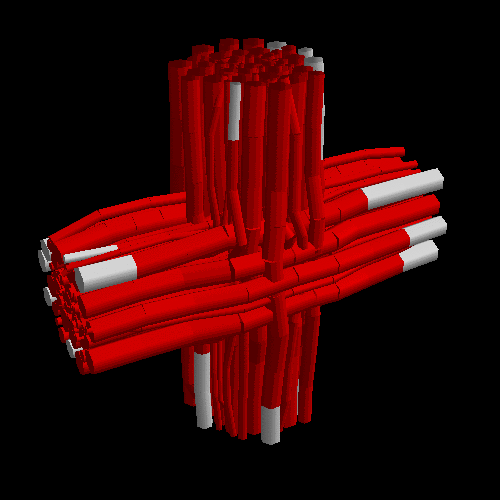
\includegraphics[width=\tikzwidth]{gfx/fastpli/solver-10}\hfill
    \includegraphics[width=\tikzwidth]{gfx/fastpli/solver-20}\hfill
    \includegraphics[width=\tikzwidth]{gfx/fastpli/solver-50}\hfill
    \includegraphics[width=\tikzwidth]{gfx/fastpli/solver-99}
	\caption{Exemplary visualization in the collision solving process. The red color indicates that a collision is detected in the fiber segment.}
	\label{fig:vis_solver}
\end{figure}
%
A visualization tool is available to visualize the nerve fiber configuration (see \cref{fig:vis_solver}).
This allows the user to get direct feedback (\eg{} after each step) to adjust the initial fiber configuration or boundary conditions.
It is written in \cpp{} and \ac{OpenGL} \textit{v2} \cite{isocpp, khronos}.
This implementation uses \code{gluCylinder} to represent a nerve fiber segment.
As it stands, this is by no means the fastest approach, but it is still fast enough compared to the computation time of a single step in the collision algorithm.
\par
% 
A further advanced interactive tool is also available as open source, the FAConstructor, which was developed by Jan Reuter as part of his bachelor thesis \cite{Reuter2019}.
It provides additional interactive methods for creating nerve fiber models and was written in \textit{OpenGL\,v3}.
% \par
\subsection{Transperent objects and cells}
%
\begin{figure}[!t]
    \centering
    \setlength{\tikzwidth}{0.75\textwidth}
    \inputtikz{gfx/model/vis_a}
	\caption{Generate a mesh for visualization. A mesh perpendicular to the fiber trajectory is calculated from n points. Triangles defined by these points are used as surfaces for the visualization of the object. Normal vectors can be used to smooth the visualization, and flash effects contribute to a more natural representation.}
	\label{fig:vis_mesh}
\end{figure}
%
In \cref{sec:medusa} the need of transperent objects is necesarry.
Not only the outer hull of the myelin, but also the inner axon needs to be seen in the visualization.
Additionally cells, \eg{} astrocytes, have to be visualized.
For this purpose, the former algorithm was rewritten.
For the transparent effects the algorithm needs to know the order in which the objects or triangular surfaces needs to be renderd.
This means, that the triangular surfaces have to be sorted in z-direction, \ie{} the view direction.
To order the triangular surfaces, they first have to be calculated.
The fiber segments are no longer represented as a cylinder, but as \ac{CC} which consist out of a hexagonal grid (see \cref{fig:vis_mesh}).
\par
% 
This is a huge amount of computational resources and currently a special non ye optimized case.
It is not yet included in the \ac{fastPLI} package.
The resulting visualization is shown in \cref{fig:medusa_8b}.
% 
% 
% 
\section{Medusa - sphered nerve and cell modelling}
\label{sec:medusa}
%
The algorithm described above for generating dense \ac{WM} fiber models can also be applied in \ac{dMRI}.
However, due to other imaging techniques and study priorities, other types of models are required.
\par
% 
In \ac{dMRI} the movement and interaction of water molecules with the fiber models is simulated.
When the water molecules collide with the surface of a fiber segment, the moleculs behavier, like diffusion though the surface, must be taken into account.
However, this applies not only to nerve fibers but also to other cell types.
Since the \ac{WM} consists not only of axons, but also of other cells such as glial cells, astrocytes and olegodendrites, these are also changing the signal of the \ac{dMRI}.
\par
% 
Therefore, an additional algorithm was developed in collaboration with Kevin Ginsburger and Cyril Poupon (Neurospin, \ac{CEA}).
This algorithm called \ac{MEDUSA} \cite{Ginsburger2019} works similarly to the algorithm described above, but models the 3d objects as spheres rather than pipe segments.
This has the advantage that the objects are simpler, which leads to an increase in collision detection, but spheres are able to approximate a 3d object like a cell body.
The latter is achieved by representing the surface of a cell body as the sum of several spheres. 
The resulting total surface of all spheres represents the cell (see \cref{ig:medusaCell}).
In this way, very complicated shapes are possible.
\par
%  
A major feature of this algorithm is how to construct other cell types and, in particular, olegodendrites whose arms connect to the myelin layer of a nearby axon.
Another focus is on the internal configurations of the cells.
Nerve fibers are initialized as fiber populations with parameters such as density and angular dispersion \cite[Ginsburger2019, ginsburgerDis2019].
Analogous to the \cref{sec:Solver} algorithm, the collisions of the objects are then checked and slowly pushed forward until no more collisions can be detected.
This algorithm is then capable of generating extensive libraries of fiber models with varying numbers of individual fiber populations (see \cref{fig:medusa_8a}).
\par
% 
The disadvantage of the spheres is that for the representation of tubular objects many more spheres and thus objects for collision control are needed.
Since the number ob objects, \ie{} spheres, is so much higher, the algorithm was implemented on the \ac{GPU} with a axes aligned bounding box search algorithm \cite{Karras2012}.
% 
% 
%
\subsection{Algorithm}
%
\begin{figure}[!t]
    \centering
    \setlength{\tikzwidth}{0.75\textwidth}
    \subcaptionbox{modified from \cite{Ginsburger2019}. Outer blue spheres myelin, inner red spheres axon}[0.75\textwidth]{
    \inputtikz{gfx/model/medusa/medusa_spheres}}
    \\[2em]
    % 
    \subcaptionbox{Cell aproximation by overlapping spheres.}[0.75\textwidth]{
    \inputtikz{gfx/model/medusa/medusa_cells}}
    \caption{\ac{MEDUSA} sphere approximation.}
    \label{fig:medusaCell}
\end{figure}
%
Since all objects are represented as a collection of spheres (see \cref{fig:medusaCell})
\begin{align}
    \mathcal{S} = \{ (x_i,y_i,z_i,r_i) : i \in \{0, 1, ..., n_\text{objects}-1\}  \}
\end{align}
%
, a collision occurs when
%
\begin{align}
d<r_i+r_j \enspace \text{with} \enspace d = \abs{\vec{p}_i - \vec{p}_j}
\end{align}
%
However, since adjacent spheres in a fiber collide when the fiber is densely populated, they must be excluded if the length of the partial trajectory is smaler then the sum of the radii of the two spheres:
\begin{align}
\text{ignore if} \enspace \sum_{n=i}^{j-1} \, \abs{\vec{p}_n - \vec{p}_{n+1}} \leq  r_i + r_j 
\end{align}
%
Spheres inside cell bodies are not checked for collisions because their volume is approximately equal to the volume of the cell.
\par
%
The calculation of the collisions is performed using the GPU architecture.
For this first implementation, the algorithm \name{AxisAligedSortedSearch} \cite{Karras2012} is used.
It sorts the spheres along an axis, \obda{} x-axis, and for each sphere $i$ searches for the first and last possible collision on that axis.
This results in a list of balls $\mathcal{C}_i$ to be tested:
\begin{align}
\begin{split}
\mathcal{C}_i = \{ s \in \mathcal{S} \mid \abs{s_i.x - s_j.x} < r_i+r_j \}
\end{split}
\end{align}
%
\begin{lstfloat}[!t]
	\lstinputlisting[style=cpp]{code/medusa.cu}
	\caption{Pseudocode of \acs{MEDUSA}s collision checking.}
	\label{alg:medusa_collision}
\end{lstfloat}
%
The algorithm described above is currently used for volumes of about $\SI{200}{\micro\meter}$ for different number of fiber populations and other properties (see \cref{fig:medusa_8a}).
For this volume size, the algorithm is fast enough for current use.
However, there are more advanced algorithms that can be used here.
One promising technique is to use a \name{BoundindBoxHierarchy} \cite{Karras2012}.
%
\begin{figure}[!t]
    \centering
    \subcaptionbox{Cubic volumes with different number pf fiber populations and volume fractions (VF) are generated.}[0.75\textwidth]{\label{fig:medusa_8a}
    \resizebox{0.75\textwidth}{!}{
    \includegraphics{gfx/model/medusa/8.jpg}}}
    \\[2em]
    \subcaptionbox{Exemplary visualization of a volume filled with a single fiber population and astrocytes.}[0.75\textwidth]{\label{fig:medusa_8b}
    \resizebox{0.75\textwidth}{!}{
    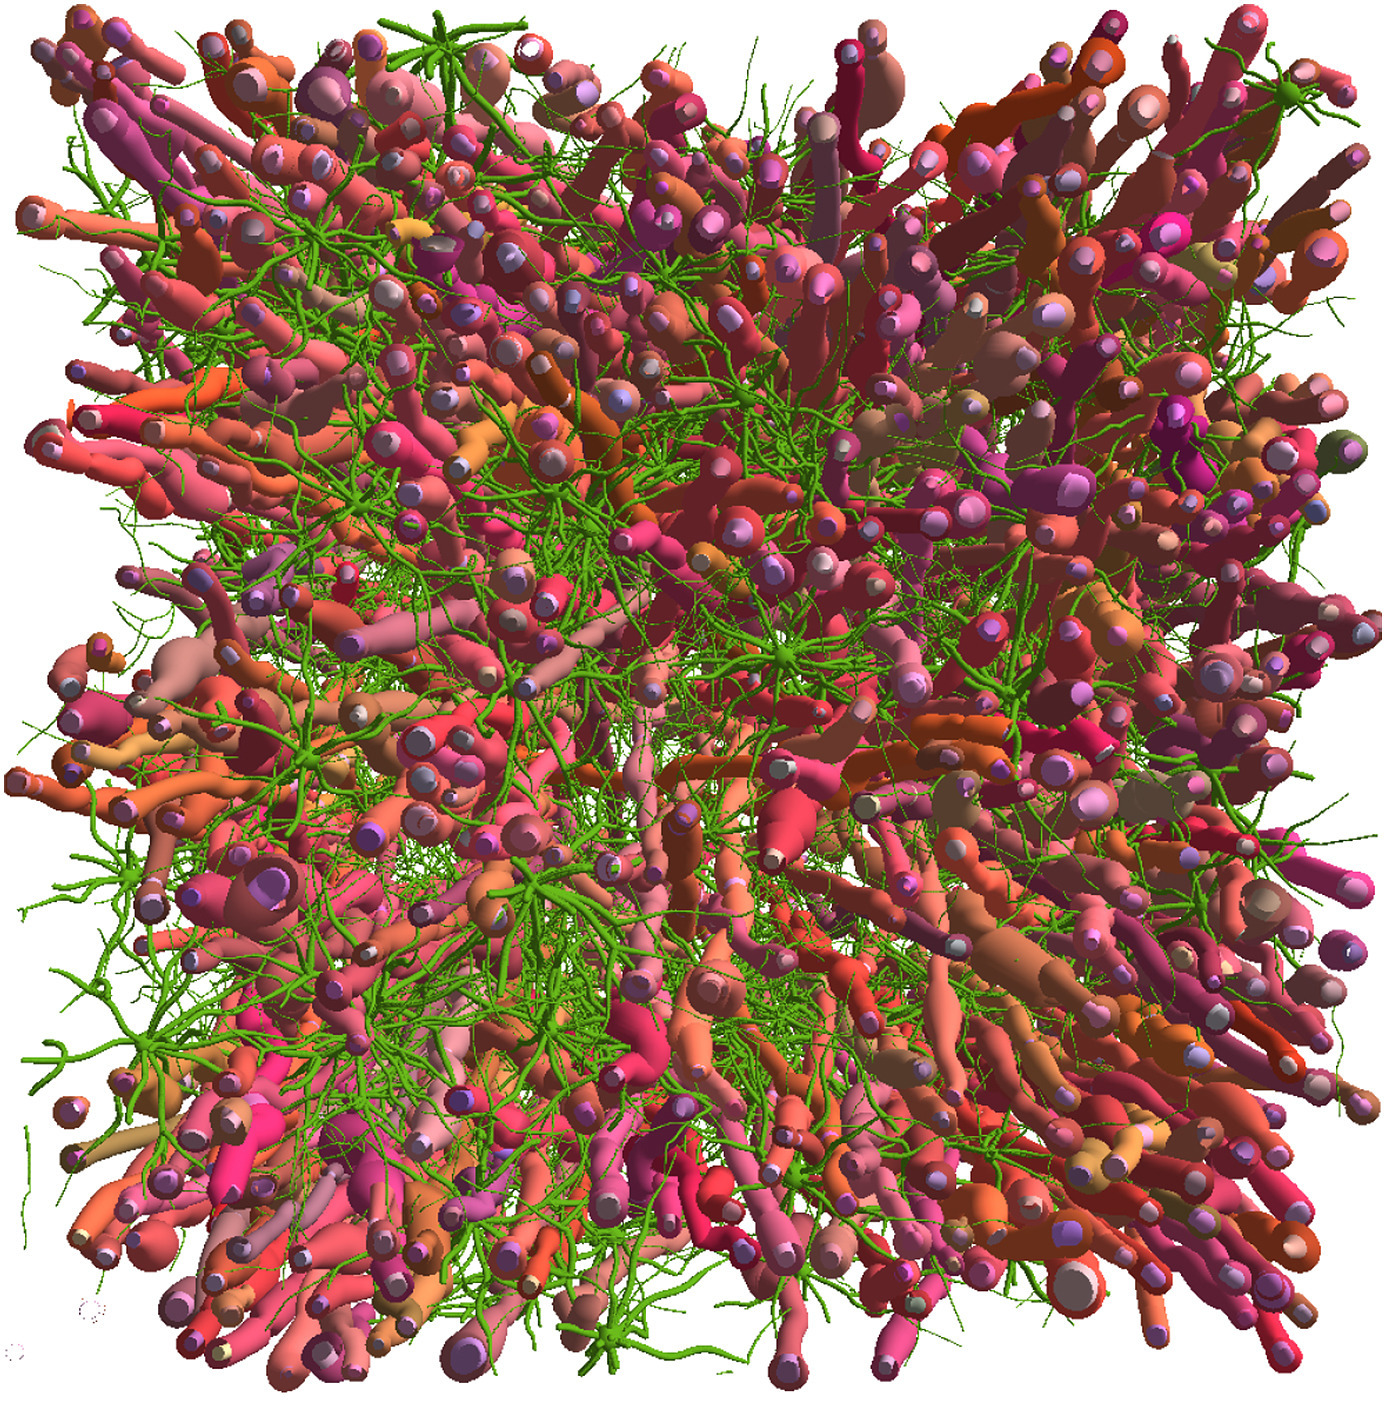
\includegraphics{gfx/model/medusa/11_.jpg}}}
	\caption{Original images from \cite{Ginsburger2019}.}
	\label{fig:medusa_8}
\end{figure}
% 
% 
% 
% \subsection{Visualization of transperent objects}
% % 
% \begin{figure}[!t]
%     \centering
%     \setlength{\tikzwidth}{0.75\textwidth}
%     \inputtikz{gfx/model/vis_a}
% 	\caption{Generate a mesh for visualization. A mesh perpendicular to the fiber trajectory is calculated from n points. Triangles defined by these points are used as surfaces for the visualization of the object. Normal vectors can be used to smooth the visualization, and flash effects contribute to a more natural representation.}
% 	\label{fig:vis_mesh}
% \end{figure}
% % 
% \todo{write}